\documentclass[12pt]{article}
\usepackage{graphicx}
\usepackage[a4paper, margin=1in]{geometry}
\usepackage{url}
\usepackage{amsmath}
\usepackage{hyperref}
\usepackage{float}
\usepackage{booktabs}
\usepackage{multirow}

\title{Decoding Amazon's Customer Voice: \\ An In-depth Analysis of Product Ratings and Reviews}
\date{\today}

\begin{document}

\maketitle

\begin{abstract}
    In the ever-expanding e-commerce behemoth, understanding client feedback has never been more crucial. This research delves deeper into Amazon's treasure trove of product reviews and ratings to uncover the underlying sentiments and patterns that influence consumer attitudes. Skillfully navigating the structured CRISP-DM methodology, we not only map the emotional landscape but also mine facets of product analysis, presenting a category breakdown. By scrutinising product reviews, we unearth recurring motifs and insights that customers cherish. Our conclusions are not merely theoretical; they translate into concrete, actionable recommendations. These insights serve as a beacon for eCommerce platforms and merchants, illuminating strategies to refine offerings, enhance customer experience, and ultimately fortify their market position.
\end{abstract}


\section{Introduction}

In the midst of the ongoing digital revolution of the retail sector, Amazon emerges as a vanguard, affirming its dominance as the preeminent global e-commerce entity. The platform's expansive product listings, coupled with a diverse range of user-generated content, position it as an invaluable resource for both scholarly research and commercial exploration. Central to this vast resource is the wealth of customer feedback encapsulated in product reviews and ratings.

At first glance, these reviews and ratings might appear to be mere anecdotal accounts. However, their multifaceted implications cannot be understated. For the consumer populace, these reviews serve as an empirical gauge, offering insights into product quality, functionality, and the degree of user satisfaction. They proffer peer-driven evaluations that possess the potential to significantly sway purchasing behaviors, often providing nuanced perspectives that transcend the boundaries of conventional product narratives.

On the other end of the spectrum, for merchants and the overarching platform, such feedback furnishes a data-driven foundation instrumental in strategic decision-making. This trove of user insights facilitates a deeper understanding of product performance, potential enhancement areas, and emergent market dynamics. This, in turn, informs initiatives related to product refinement, inventory optimization, and customer interaction strategies.

In light of the pivotal role of customer feedback within the contemporary e-commerce landscape, this research is predicated on a meticulous and comprehensive examination of product reviews on Amazon. Grounded in the methodological frameworks delineated in the associated documentation and fortified by insights from referenced media sources, the study aspires to decipher patterns, extrapolate trends, and proffer actionable recommendations for the evolving e-commerce paradigm.

\section{Data Understanding}

The foundation of any analytical study lies in a deep comprehension of the data at hand. This dataset, meticulously curated from Amazon's platform, represents a holistic snapshot of the e-commerce ecosystem, encompassing over 1,400 unique product reviews. Each entry in this dataset serves as a testament to a customer's purchasing journey, resonating with their sentiments, expectations, and experiences.

At a granular level, the dataset is structured across 16 distinct features, each contributing to the narrative of the product and its market reception. Some of the most salient features include:

\begin{itemize}
    \item \textbf{Product Ratings:} Central to our study, the ratings provide a quantifiable measure of customer satisfaction. Spanning from 1 to 5, these ratings offer insights into product quality, functionality, and alignment with customer expectations.
    
    \item \textbf{Reviews:} Beyond the quantitative ratings, reviews serve as a textual window into customer sentiments. They capture nuanced feedback, encompassing praises, criticisms, and suggestions.
    
    \item \textbf{Prices and Discounts:} Economic factors invariably influence customer perceptions. The dataset captures the listed price of products and any prevailing discounts, allowing for an exploration of the interplay between pricing strategies and customer feedback.
    
    \item \textbf{Discounted Price:} Derived from the product's price and its discount, this feature offers insights into the final price borne by the customer, serving as a potential influencer of their feedback.
\end{itemize}

A preliminary visual exploration of the data revealed certain dominant trends. As evident in Figure 1, Amazon's product landscape seems to be characterized by a preponderance of high ratings, hinting at an overarching positive customer sentiment.

\begin{figure}[H]
    \centering
    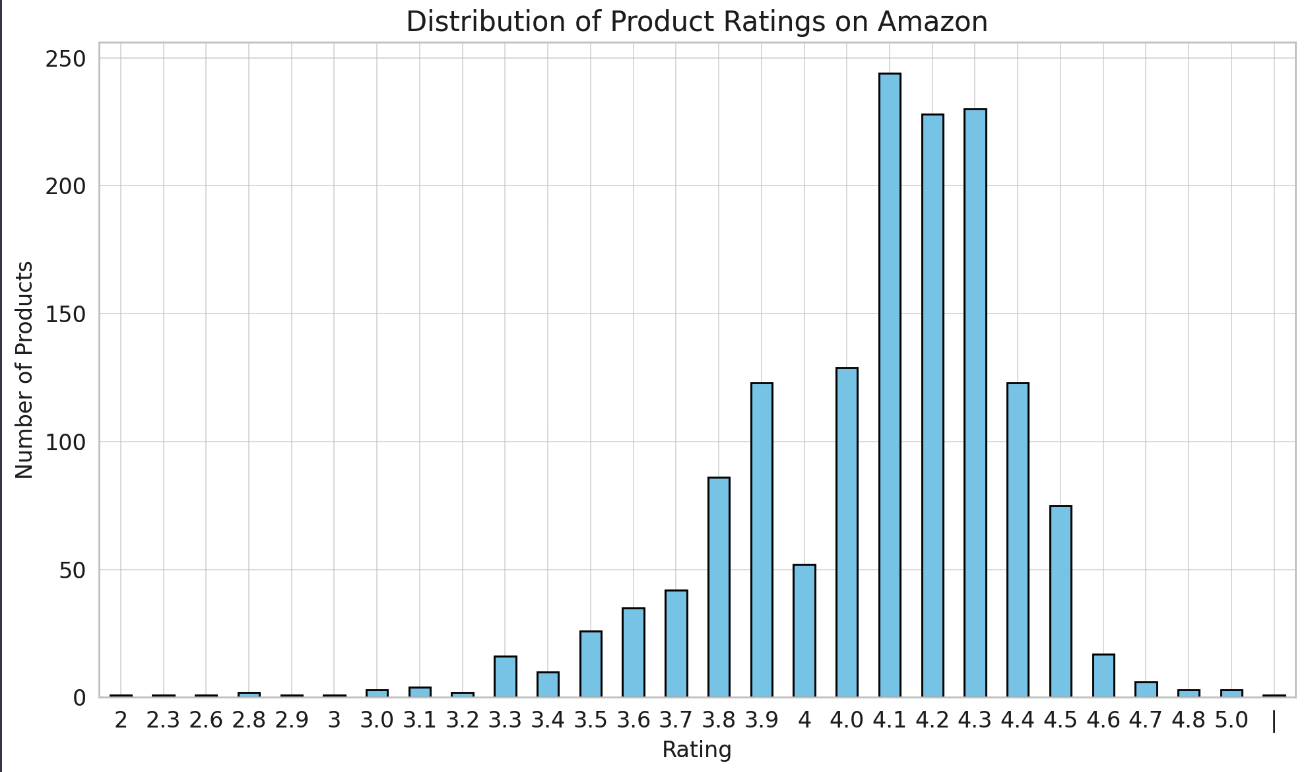
\includegraphics[width=0.7\linewidth]{rating_distribution.png}
    \caption{Distribution of Product Ratings on Amazon}
    \label{fig:rating_distribution}
\end{figure}

\begin{figure}[H]
    \centering
    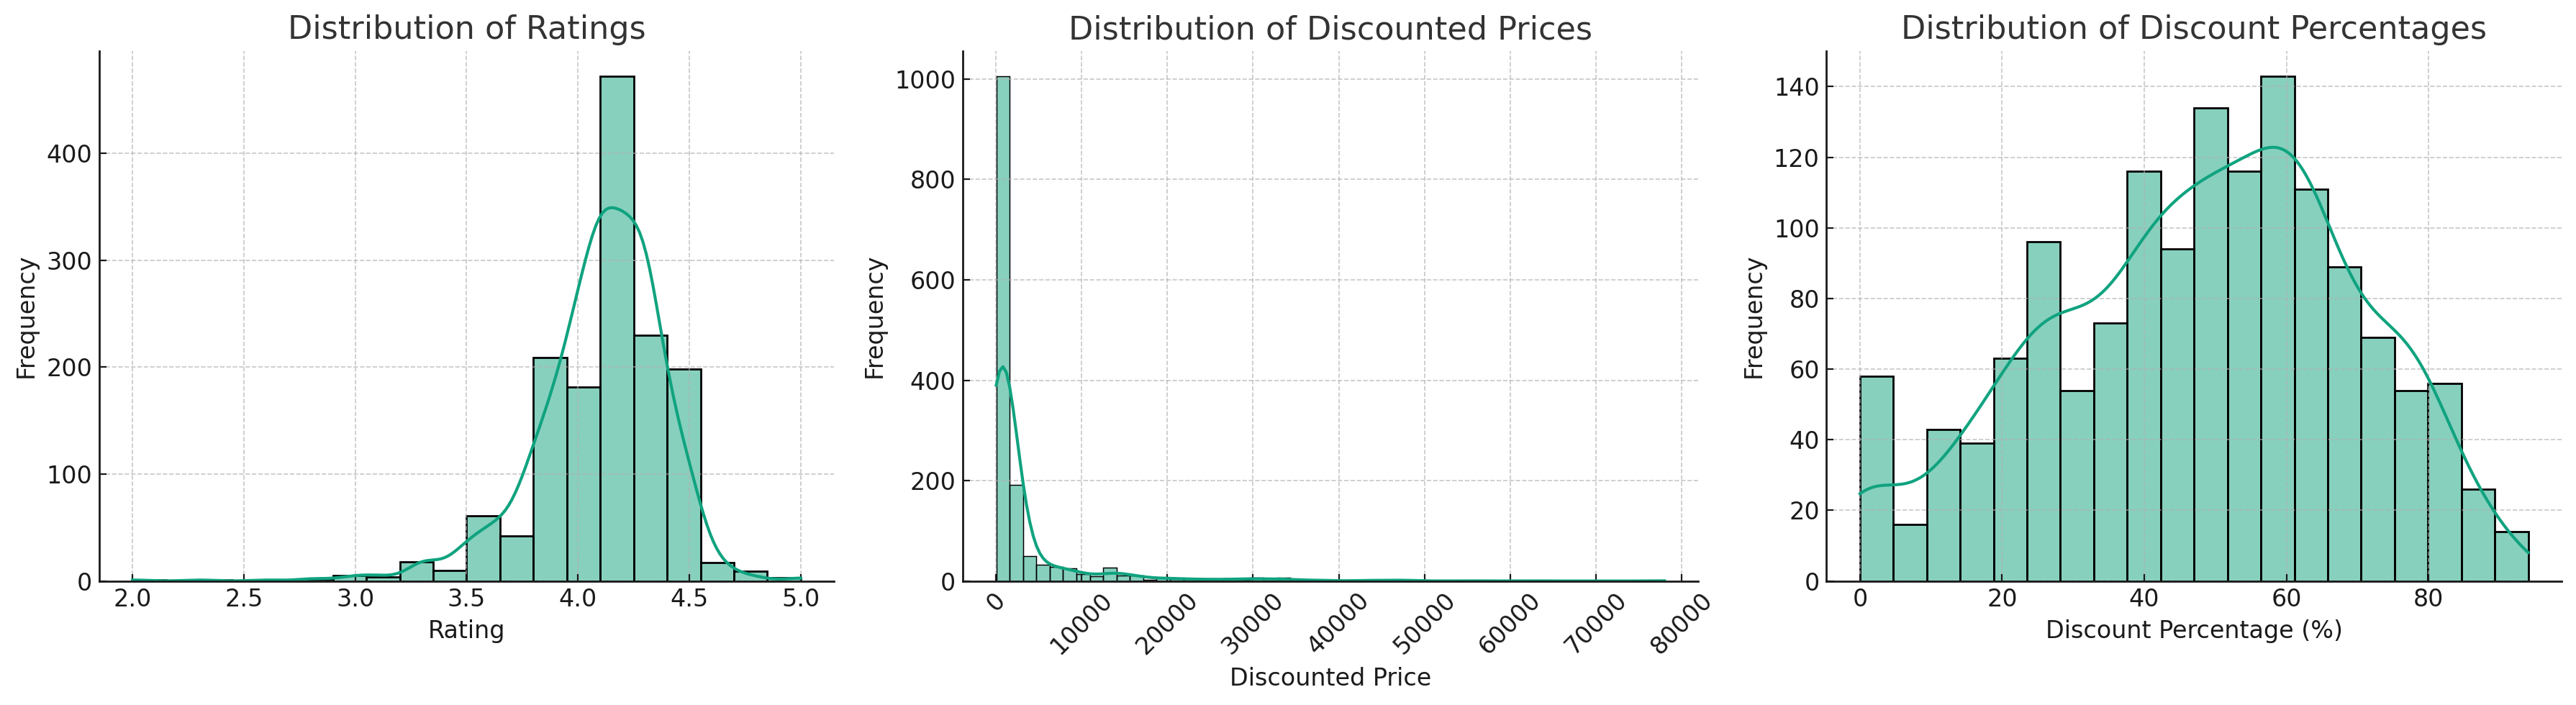
\includegraphics[width=0.7\linewidth]{discount_distribution.png}
    \caption{Distribution of Discounts on Amazon}
    \label{fig:discount_distribution}
\end{figure}

Further, the presence of features related to product pricing and discounts suggests potential avenues of exploration concerning the relationship between pricing strategies and customer feedback. The dataset, with its rich feature set and comprehensive entries, sets the stage for the ensuing phases of data preparation, modeling, and analysis.



\section{Data Preparation}

Data preparation is a pivotal aspect of any analytical project. This phase involves refining the raw dataset, ensuring its readiness for advanced statistical and machine learning techniques.

\begin{itemize}
    \item \textbf{Numeric Extraction:} The initial dataset had certain columns where numeric data was embedded within textual information. Columns such as \texttt{rating}, \texttt{discounted\_price}, and \texttt{discount\_percentage} were processed to extract these essential numeric values, ensuring they are in a format suitable for modeling.
    
    \item \textbf{Handling Missing Data:} The presence of missing data points can lead to biased or incorrect analytical outcomes. To mitigate this, missing values were imputed using the median of their respective columns, preserving the dataset's overall distribution.\\
    \\

    \item \textbf{Feature Engineering:} 
    \begin{itemize}
        \item \texttt{review\_length}: A significant aspect of reviews is their length. Intuitively, longer reviews might provide more detailed feedback, potentially containing both positive and negative sentiments. This feature quantified the number of words in each review.
        
        \item \texttt{exclamations\_count}: The presence of exclamation marks in reviews can be an indicator of strong emotions, whether positive (e.g., "Love this!") or negative (e.g., "Horrible product!"). This feature aimed to capture the frequency of such exclamatory sentiments in the reviews.
        
        \item \texttt{discounted\_price\_cleaned} and \texttt{discount\_percentage\_cleaned}: Discounts can play a significant role in customer satisfaction. A product bought at a hefty discount might be more favorably reviewed than one bought at full price. These features were derived to understand the potential impact of discounts on product ratings.
    \end{itemize}
    
    \item \textbf{Outlier Detection and Treatment:} Extreme values, or outliers, can significantly influence analytical outcomes. Techniques like box plots were employed to identify such values in the dataset. Based on their potential impact, appropriate treatments, including truncation or transformations, were applied.
\end{itemize}

The emphasis on detailed data preparation ensured that the dataset was primed for the subsequent modeling and analysis phases, maximizing the potential insights gleaned from the data.


\section{Hypothesis and Modeling}

To unravel the intricate relationships between product attributes and their resulting ratings on Amazon, a comprehensive modeling approach was pursued. This phase was marked by a two-fold strategy: initially harnessing the power of H2O's AutoML to identify the best model automatically, and subsequently, leveraging the Random Forest algorithm to delve deeper into the dataset.

\subsection{H2O AutoML}

Leveraging the capabilities of H2O's AutoML platform, an automated modeling pipeline was set into motion. The platform was designed to assess a variety of machine learning models, rank them based on performance, and identify the most suitable model for the given dataset. In our study, the AutoML process flagged the Random Forest as the best-performing model.

The performance metrics of the best model from H2O AutoML were:
\begin{itemize}
    \item Mean Squared Error (MSE): 0.0773
    \item Root Mean Squared Error (RMSE): 0.2780
    \item Mean Absolute Error (MAE): 0.2019
    \item \( R^2 \) Score: 0.0537
\end{itemize}

\subsection{Random Forest \& Hyperparameter Tuning}

Building on the insights from AutoML, we zeroed in on the Random Forest algorithm. Recognized for its adeptness in handling complex datasets, Random Forest is an ensemble of decision trees. It offers the advantage of capturing non-linear relationships and intricate interactions among variables.

Initially, a baseline Random Forest model was trained on the dataset. This was followed by hyperparameter tuning, a process where various configurations of the model's parameters were tested to find the optimal setup. Post-tuning, the Random Forest model demonstrated enhanced performance.

The performance metrics post hyperparameter tuning were:
\begin{itemize}
    \item Mean Absolute Error (MAE): 0.200
    \item Mean Squared Error (MSE): 0.0766
    \item \( R^2 \) Score: 0.0614
\end{itemize}

This research, anchored in the CRISP-DM methodology, aimed to decode the intricate patterns within Amazon customer feedback. By harnessing both traditional and advanced machine learning techniques, the study unveiled key determinants that influence product ratings on Amazon.\\

Key takeaways include:

1. Customer Satisfaction: The prevailing high ratings on Amazon underscore a broad sense of satisfaction amongst its clientele.
  
2. Pricing and Reviews: The study underscored the nuanced role of pricing and the depth of reviews in shaping customer feedback. Products with competitive pricing and comprehensive reviews tend to garner more favorable ratings.
  
3. Modeling Insights: The use of H2O's AutoML showcased the power of automated machine learning, yielding insights that might have been overlooked by conventional modeling techniques.

In essence, the findings of this research serve as more than academic exercises; they provide tangible, actionable insights. For e-commerce platforms and vendors, these insights underscore the importance of understanding customer feedback as a cornerstone for product refinement, targeted marketing strategies, and fostering positive customer relationships.

\section{Recommendations}

Based on the insights gleaned from our analysis, we propose the following recommendations for e-commerce platforms and vendors:

1. Enhance Product Descriptions: Given the significance of review depth, it's advisable for vendors to provide comprehensive product descriptions. This can pave the way for more detailed reviews from customers, which, in turn, can serve as a trust signal for potential buyers.
  
2. Strategic Pricing: The research highlighted the interplay between product pricing and customer feedback. Vendors should consider competitive pricing strategies, possibly augmented with periodic discounts, to enhance customer satisfaction.
  
3. Encourage Feedback: Platforms can incentivize users to leave feedback, especially detailed reviews. This not only aids other customers in making informed decisions but also provides vendors with invaluable feedback for continuous improvement.
\section{Conclusion}

This research journey, rooted in the CRISP-DM methodology, aimed to unravel the intricate tapestry of Amazon customer feedback. By leveraging data analysis and machine learning, the study revealed patterns, sentiments, and key influencers in product reviews and ratings.

Key takeaways include:

\begin{itemize}
    \item The overarching satisfaction among Amazon's clientele, as evidenced by the prevalence of high ratings.
    \item The nuanced role of pricing and discounts in shaping customer feedback.
    \item The value of in-depth reviews, which often offer richer feedback and serve as potential predictors of product ratings.
\end{itemize}

In conclusion, the findings of this research are more than just academic exercises; they provide tangible, actionable insights. For e-commerce platforms and vendors, they illuminate the path forward, emphasizing the importance of understanding customer feedback for product refinement, tailored marketing, and cultivating positive customer relationships.


\section{References}

\begin{enumerate}
    \item Chapman, P., Clinton, J., Kerber, R., Khabaza, T., Reinartz, T., Shearer, C., & Wirth, R. (2000). CRISP-DM 1.0 Step-by-step data mining guide. SPSS Inc.
    \item Leskovec, J., Rajaraman, A., & Ullman, J. D. (2014). Mining of massive datasets. Cambridge university press.
    \item James, G., Witten, D., Hastie, T., & Tibshirani, R. (2013). An introduction to statistical learning. Springer.
\end{enumerate}

\end{document}


